\documentclass[brazil, a4paper, 14pt]{article}

\usepackage[brazil]{babel}
\usepackage[utf8]{inputenc}
\usepackage{fancyhdr}
\usepackage{graphicx}
\graphicspath{ {./imagens/} }
\usepackage{geometry}
\usepackage[utf8]{inputenc}
\usepackage{kpfonts}
\usepackage[T1]{fontenc}
\usepackage{url}
\usepackage{hyperref}
\usepackage{listings}
\usepackage{indentfirst}
\usepackage{titlesec}
\newcommand{\sectionbreak}{\clearpage}
\usepackage[usenames]{color}
\usepackage{multicol}
\usepackage{wrapfig}
\usepackage{array}
\usepackage{makecell}
\usepackage{booktabs}
\usepackage{multirow}
\usepackage{verbatim}
\usepackage{enumitem}
\usepackage{pdfpages}
\usepackage{float}
\usepackage{forest}
\usepackage{datetime}
\usepackage{minted}
\usepackage{pmboxdraw} % for box drawings
\usepackage{fancyvrb}
\usepackage{tgcursor}

% Formating source code
\definecolor{c3green}{RGB}{174,201,0}
\definecolor{c3gray}{rgb}{0.21, 0.27, 0.31}
\lstset{language=C,
    keywordstyle=\color{c3green}\bf, 
    stringstyle=\color{c3green}\it,
    commentstyle=\color{c3gray}\it,
    numbers=left,
    stepnumber=5,
    firstnumber=1,
    numberstyle=\tiny,
    extendedchars=true,
    breaklines=true,
    captionpos=b,
    tabsize=2,
    frame=single,
    basicstyle=\footnotesize,
    showstringspaces=false
}

\geometry{a4paper,left=3cm,right=2cm,top=3cm,bottom=3cm}

\pagestyle{fancy}
\fancyhf{}
\lhead{
\includegraphics[width=0.8cm]{imagens/celero_logo.jpeg}}
\rhead{Instalando Debian com criptografia}
\rfoot{Página \thepage}

\newcommand\todo[1]{\textcolor{red}{Alessandro: #1}}

%   For Shell Scripts
\setminted[bash]{
  frame=lines,
  framesep=2mm,
  baselinestretch=1.2,
  fontsize=\footnotesize,
  linenos,
  breaklines
}

\begin{document}
    \begin{titlepage}

  \begin{figure}[!ht]
    \filcenter
    
\includegraphics[height=0.33\textheight, width=0.33\linewidth, keepaspectratio]{imagens/celero_logo.jpeg}
  \end{figure}
  \vspace{-2.5em}
  \begin{Large}
      \begin{center}
        \textbf{Celero Consultoria LTDA}
  
        \vfill
  
        \textbf{Instalando Debian\\
        com criptografia
      }
    \end{center}

    \vfill
    
    \begin{center}
      Curitba\\
      23 de agosto de 2020
    \end{center}
  \end{Large}

  \clearpage
\end{titlepage}
    \tableofcontents
    
    \section{Introdução} \label{sec:intro}
Neste manual será apresentado como instalar a distribuição Linux
Debian com criptografia. Esta demanda é imprescindível, diante do
advento da lei LGPD. Instale o sistema operacional e ao final execute
o comando indicado na seção~\ref{sec:verify} e envie ao seu gestor.

\subsection{Gerando mídia de Instalação} \label{subsec:gen}
Faça o download da seguinte
iso~\href{http://ftp.br.debian.org/debian-cd/10.5.0-live/amd64/iso-hybrid/debian-live-10.5.0-amd64-gnome.iso}{debian-live-10.5.0-amd64-gnome.iso}
(este contém o sistema de instalação do sistema operacional Debian).

Utilize um pen drive para gerar a mídia de instalação. A partir de uma
distro Linux em funcionamento (peça para um colega) conecte um pen
drive em uma entrada USB com pelo menos 4GB de espaço. Execute os
seguintes comandos a partir de um terminal para gerar a mídia de instalação:\\

\textcolor{red}{(mas tome cuidado,
pois se gravar no dispositivo incorreto poderá danificar o sistema de
aquivos do drive incorreto).}

Execute este comando para encontrar o pen drive:
\begin{verbatim}
$ lsblk

NAME        MAJ:MIN RM   SIZE RO TYPE MOUNTPOINT
sda           8:0    0   7.5G  0 disk
└─sda1        8:1    0   7.5G  0 part 
nvme0n1     259:0    0 953.9G  0 disk 
├─nvme0n1p1 259:1    0   500M  0 part /boot
├─nvme0n1p2 259:2    0    16M  0 part 
├─nvme0n1p3 259:3    0 312.2G  0 part 
├─nvme0n1p4 259:4    0   524M  0 part 
├─nvme0n1p5 259:5    0   100G  0 part /
├─nvme0n1p6 259:6    0   220G  0 part /large_files
└─nvme0n1p7 259:7    0 320.6G  0 part /home
\end{verbatim}

Observe que neste caso \textbf{sda} é o pen drive, em outra máquina este
dispositivo poderá ser enumerado como \textbf{sdb}. \emph{Execute este
comando como usuário \textbf{root}}.

\begin{verbatim}
cat <caminho para debian-live-10.5.0-amd64-gnome.iso> > \
/dev/<drive obtido do lsblk acima>

no caso acima

cat ~/Downloads/Debian-live-10.5.0-amd64-gnome.iso > /dev/sda
\end{verbatim}

Caso não seja reportado nenhum erro o pen drive foi gerado
corretamente. \textbf{Antes de remover o pen drive certifique-se de
  que removeu-o com segurança, isso irá garantir que nada ficou em
  cache, ou seja, todos os dados foram gravados no pen drive.}
  
\subsection{Inicializando através do pen drive} \label{subsec:init}
Nesta seção é apresentado como inicializar a instalação através do
pen drive gerado na seção~\ref{subsec:gen}.

Nas máquinas Dell Inspiron (novas) você poderá pressionar a tecla F12 para
mostrar a seleção de boot (inicialização), quando ligar a máquina e
aparecer a logo da Dell pressione repetidamente F12. Caso seja uma
máquina diferente da Dell Inspiron, observe no cato superior direito o
prompt de qual tecla deve ser pressionada para seleção de boot.

Uma vez apresentado a seleção de boot, selecione o pen drive e
pressione enter, você deveria ver a tela da figura~\ref{fig:grub}:

\begin{figure}[H]
  \filcenter
  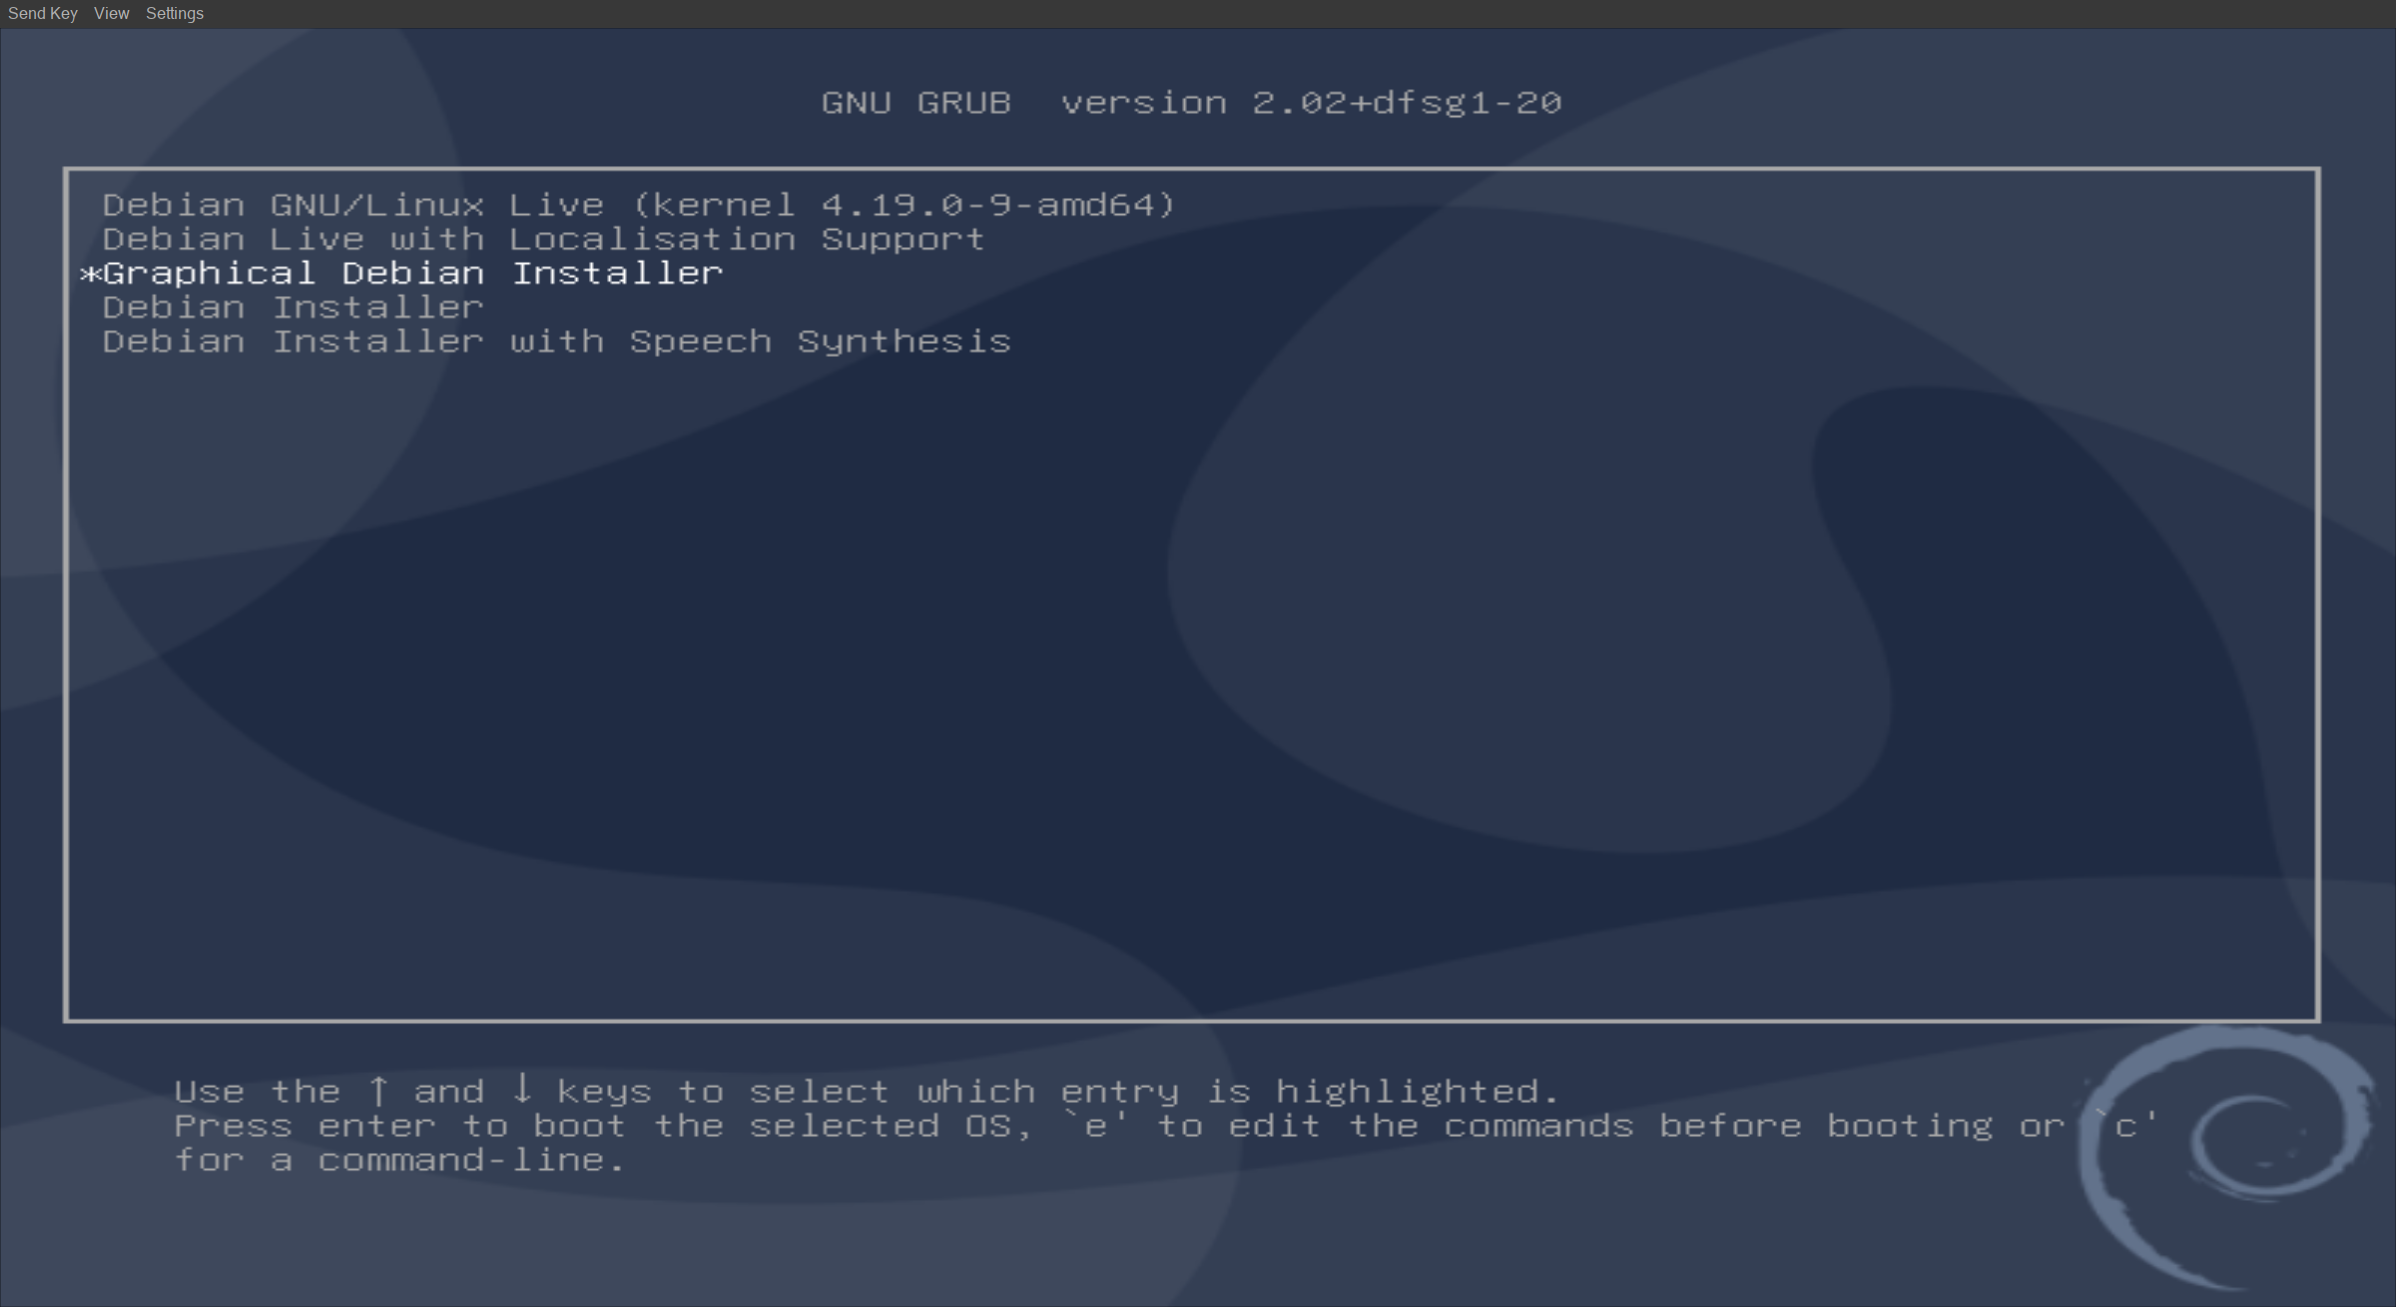
\includegraphics[height=1\textheight, width=.8\linewidth,
  keepaspectratio]{grub}
  \caption{Inicialização após seleção do pen drive.}
  \label{fig:grub}
\end{figure}


\section{Instalando com criptografia}
Nesta seção é apresentado como instalar com criptografia.

Uma vez iniciada a mídia de instalação, a primeira opção que é
apresentado é a opção de língua, selecione a desejada e siga os passos
na tela até você chegar na seguinte tela da figura~\ref{fig:lvm_encrypt}:

\begin{figure}[H]
  \filcenter
  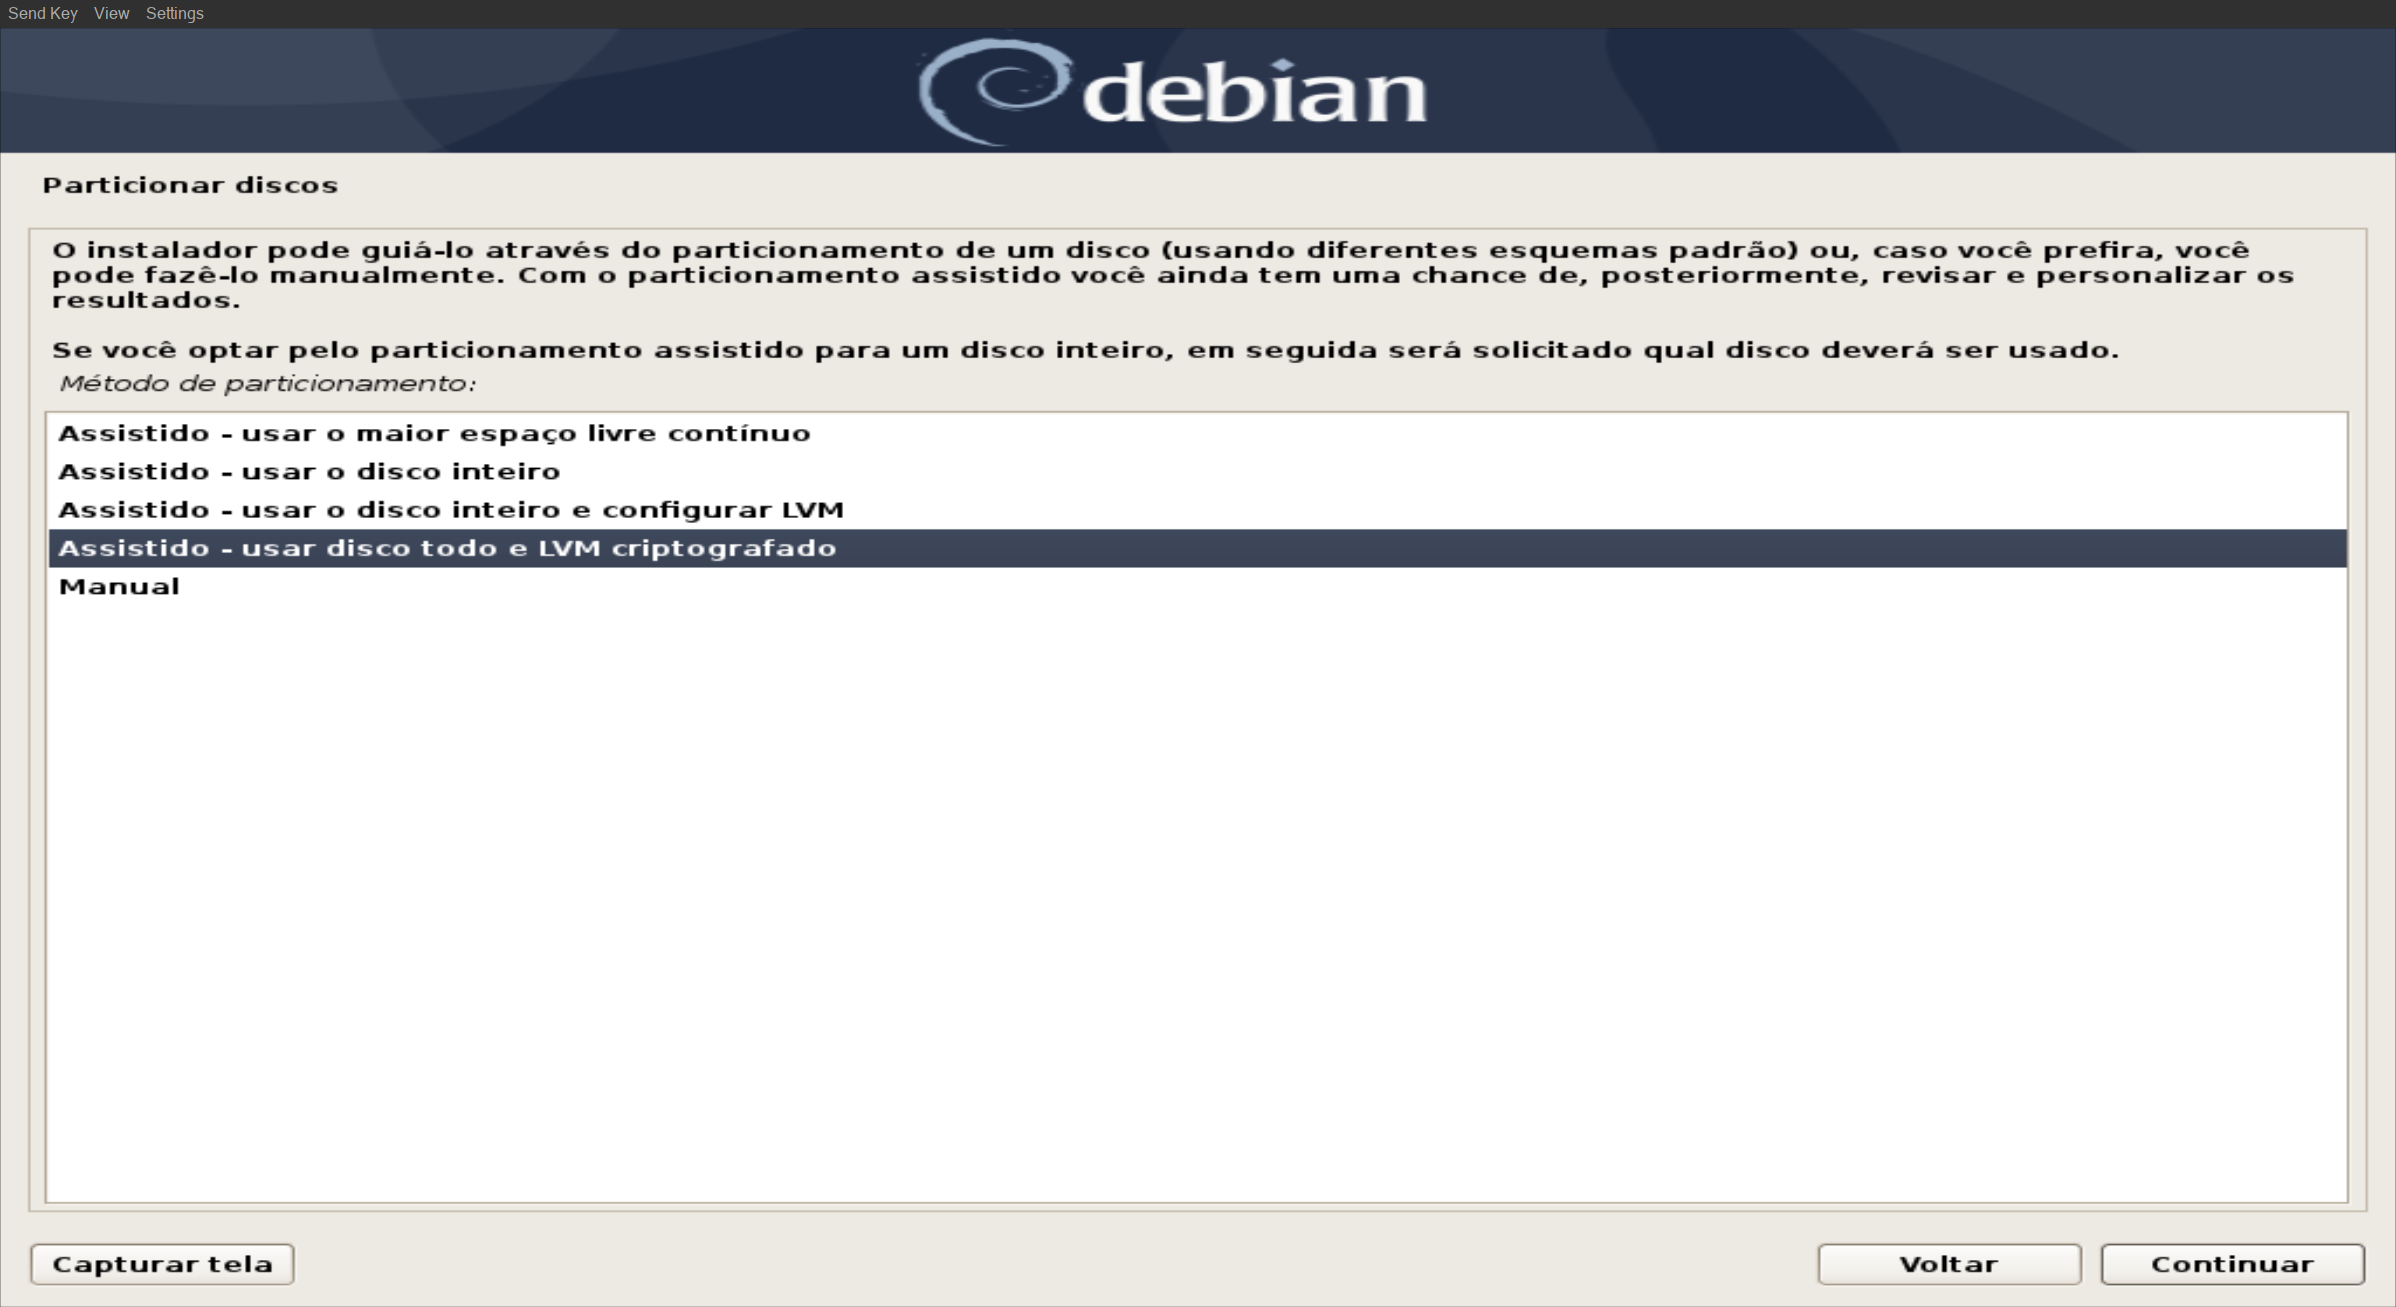
\includegraphics[height=1\textheight, width=.8\linewidth,
  keepaspectratio]{assistido-lvm-encrypted}
  \caption{Criptografar o disco todo.}
  \label{fig:lvm_encrypt}
\end{figure}

Selecione o disco que deseja instalar o sistema, caso tenha recebido
um máquina com SSD, possivelmente verá o seguinte dispositivo
\emph{nvme0n1}, se este for o caso selecione-o e siga os passos na tela.

Caso você não tenha muita experiência com instalações de sistemas
operacionais, recomendamos que selecione a opção de todos os arquivos
em uma única partição, como na tela da figura~\ref{fig:beginner}:

\begin{figure}[H]
  \filcenter
  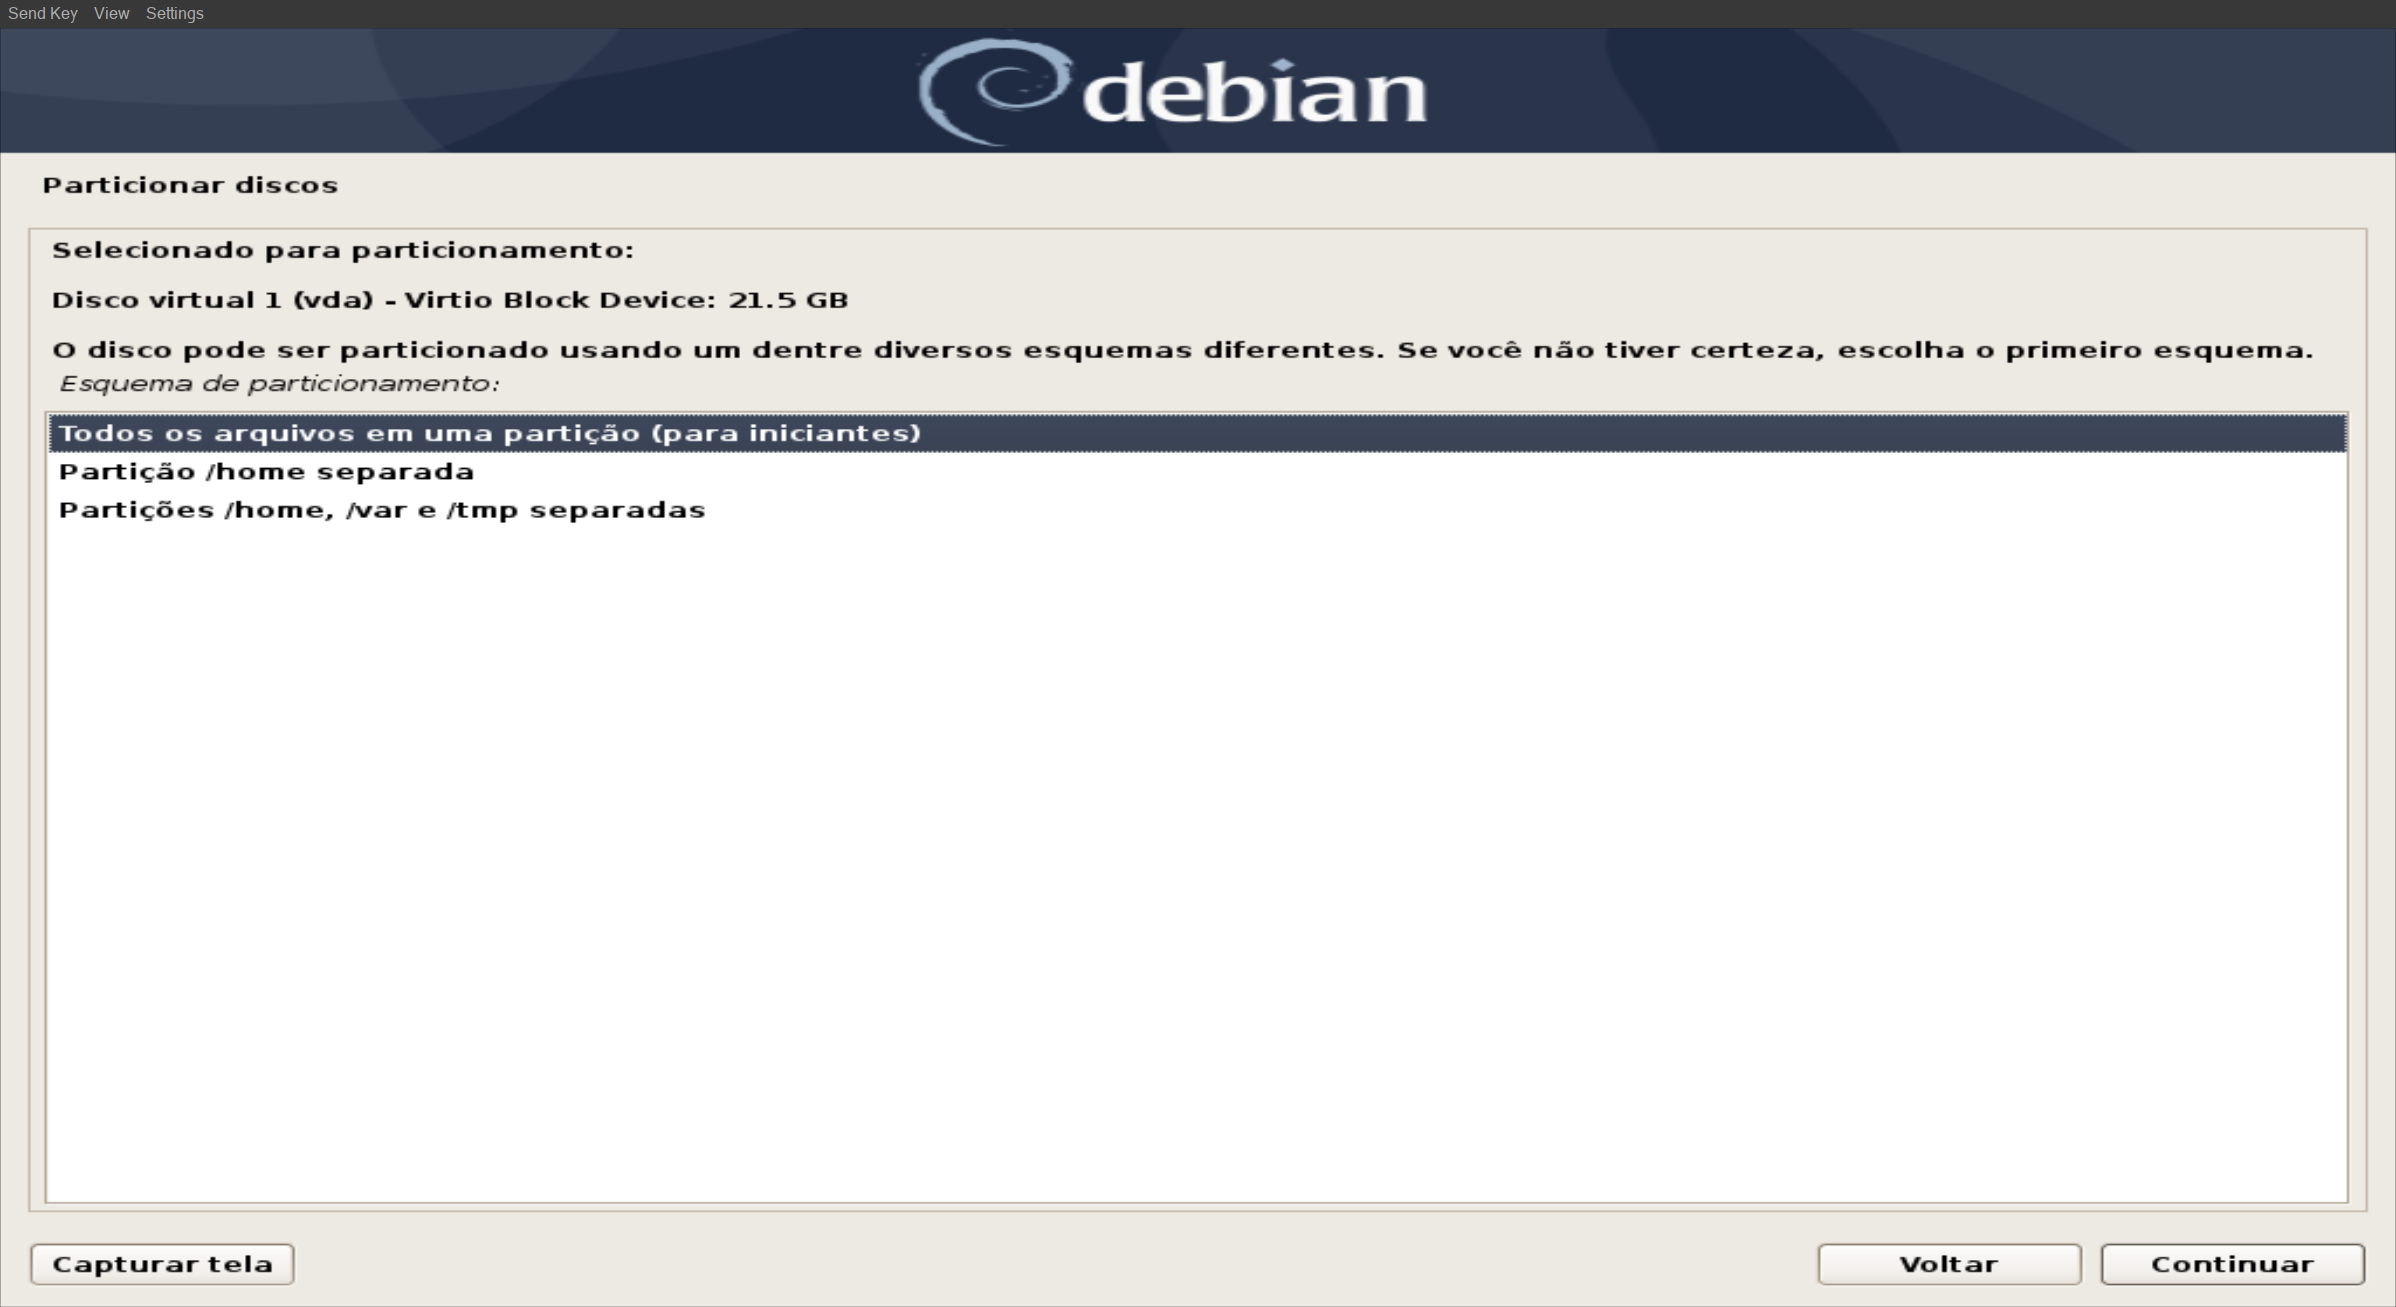
\includegraphics[height=1\textheight, width=.8\linewidth,
  keepaspectratio]{encrypt-iniciates}
  \caption{Criptografar o disco todo, para iniciantes.}
  \label{fig:beginner}
\end{figure}

Confirme que você quer gravar as partições no disco e siga os próximos
passos na tela.

O próximo passo é configurar uma senha forte\footnote{\textbf{Uma senha forte
  contem letras (maiúsculas e minusculas), números e caracteres especiais, como: \texttt{\$\&\@``''\#'}.}}

\begin{figure}[H]
  \filcenter
  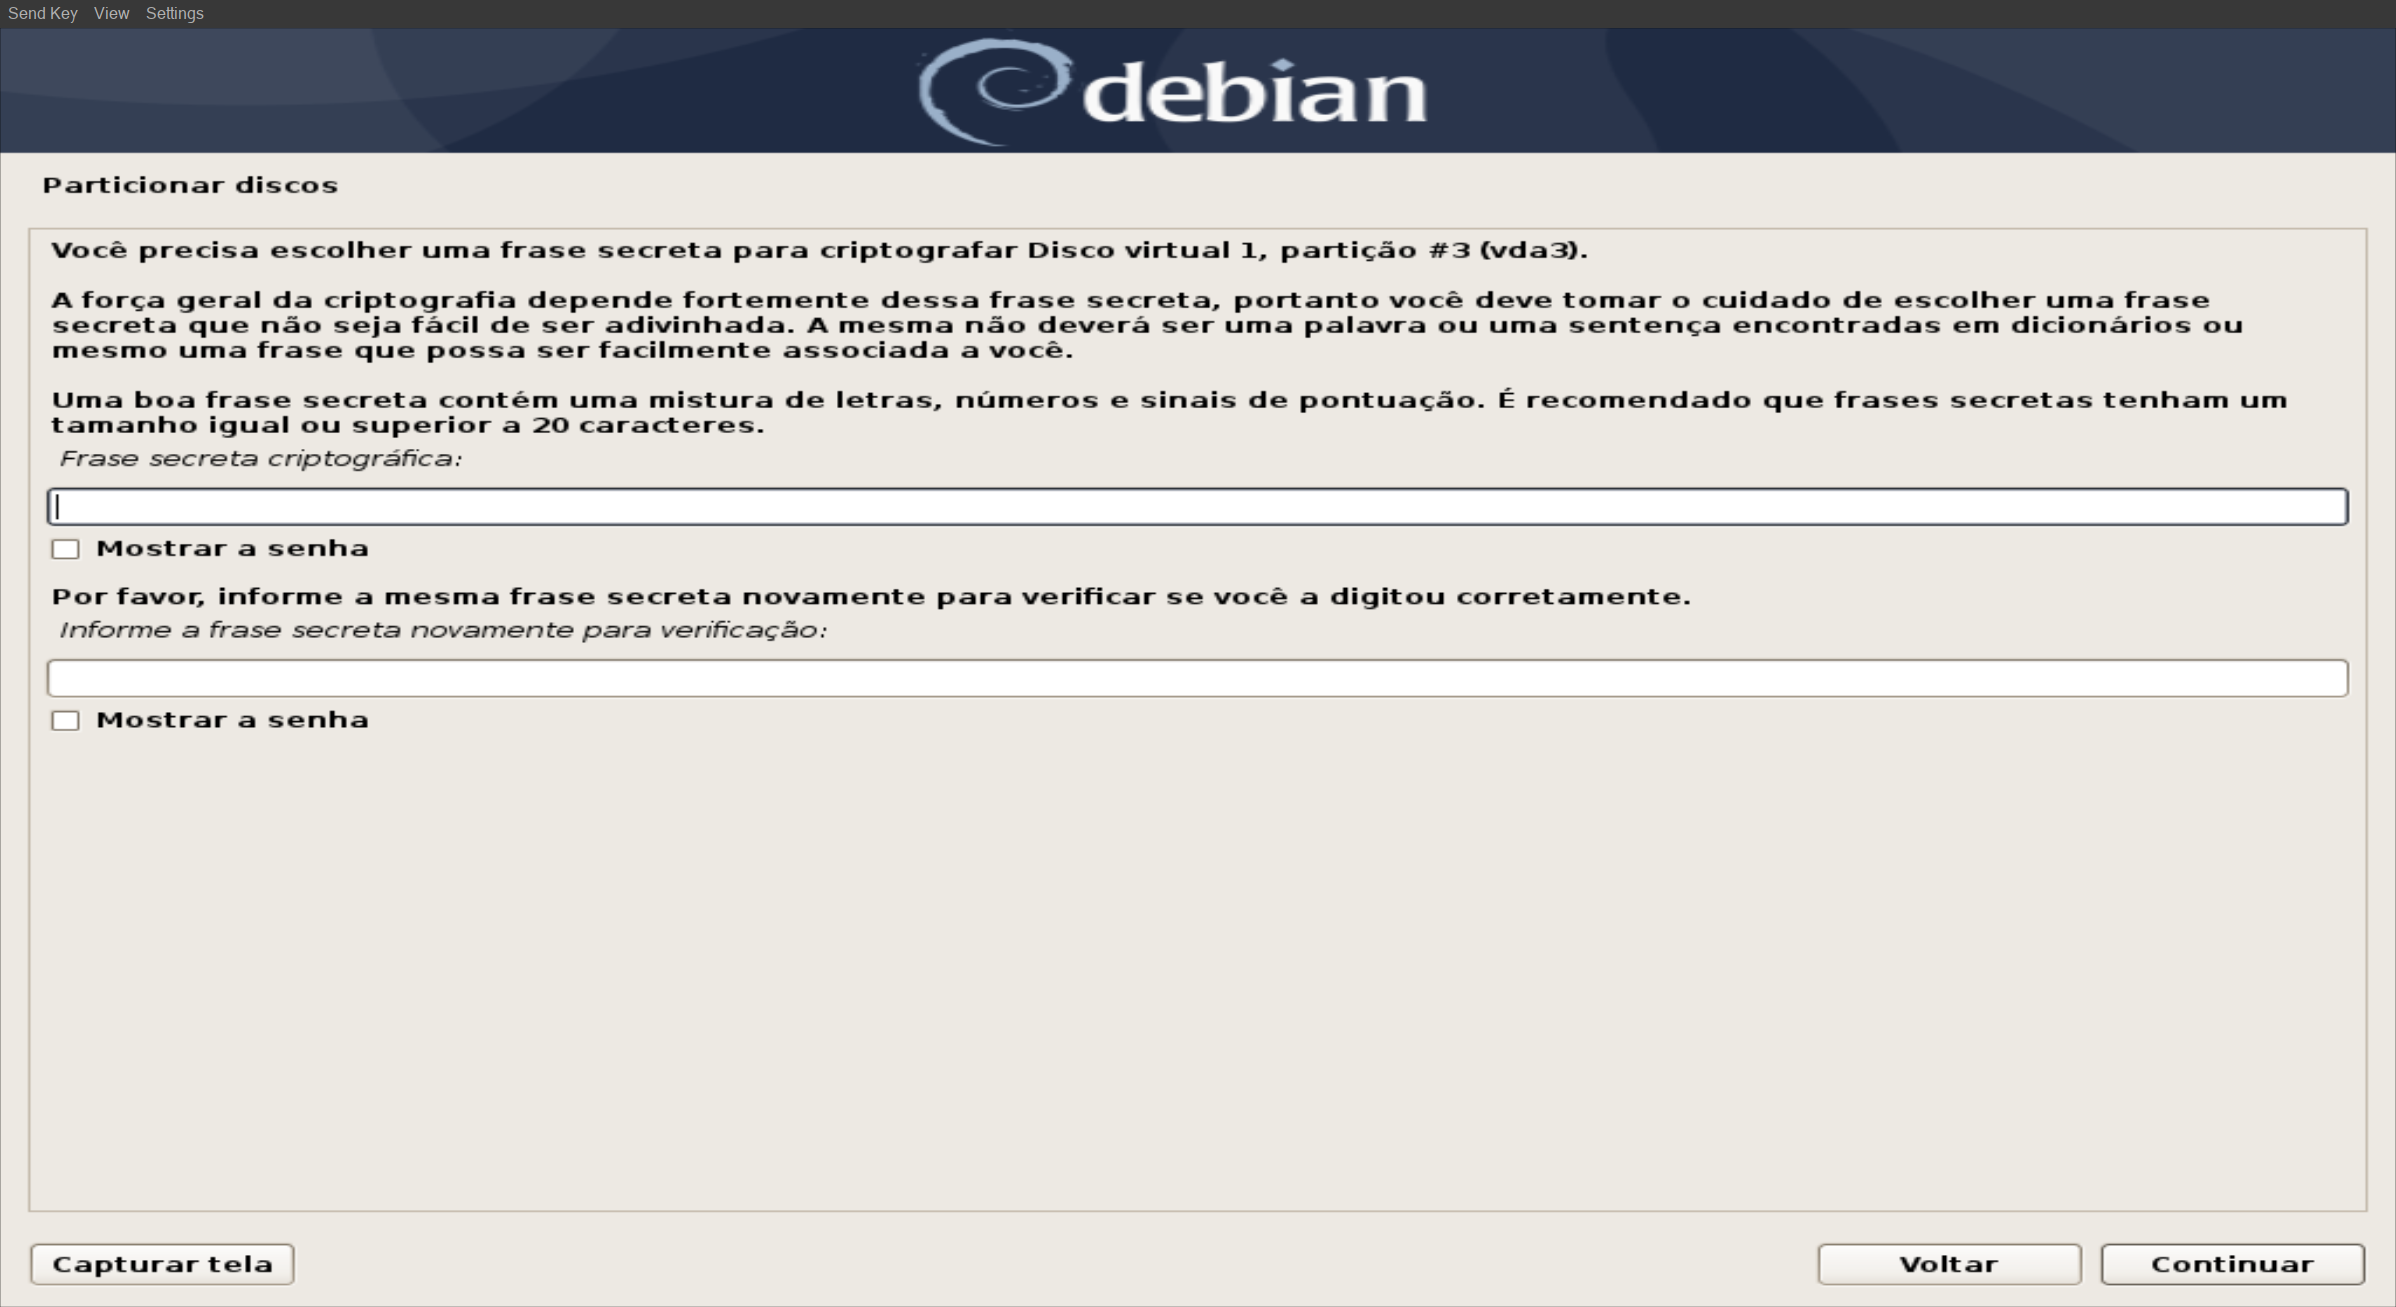
\includegraphics[height=1\textheight, width=.8\linewidth,
  keepaspectratio]{pass-encrypt}
  \caption{Configurar senha para a criptografia do disco.}
  \label{fig:pass}
\end{figure}

Uma vez configurado uma senha para a criptografia do disco, aceite o
valor padrão para utilizar todo o grupo de volume.

Por fim será apresentado um resumo de como ficará o sistema de
partições e volumes do disco, deixe selecionado ``Finalizar o
particionamento e escrever as mudanças no disco'' e pressione o botão
continuar, como mostra a figura~\ref{fig:end_encrypt}.

\textcolor{red}{\textbf{Obs: as informações apresentadas na
  figura~\ref{fig:end_encrypt} poderão variar com o seu sistema.}}

\begin{figure}[H]
  \filcenter
  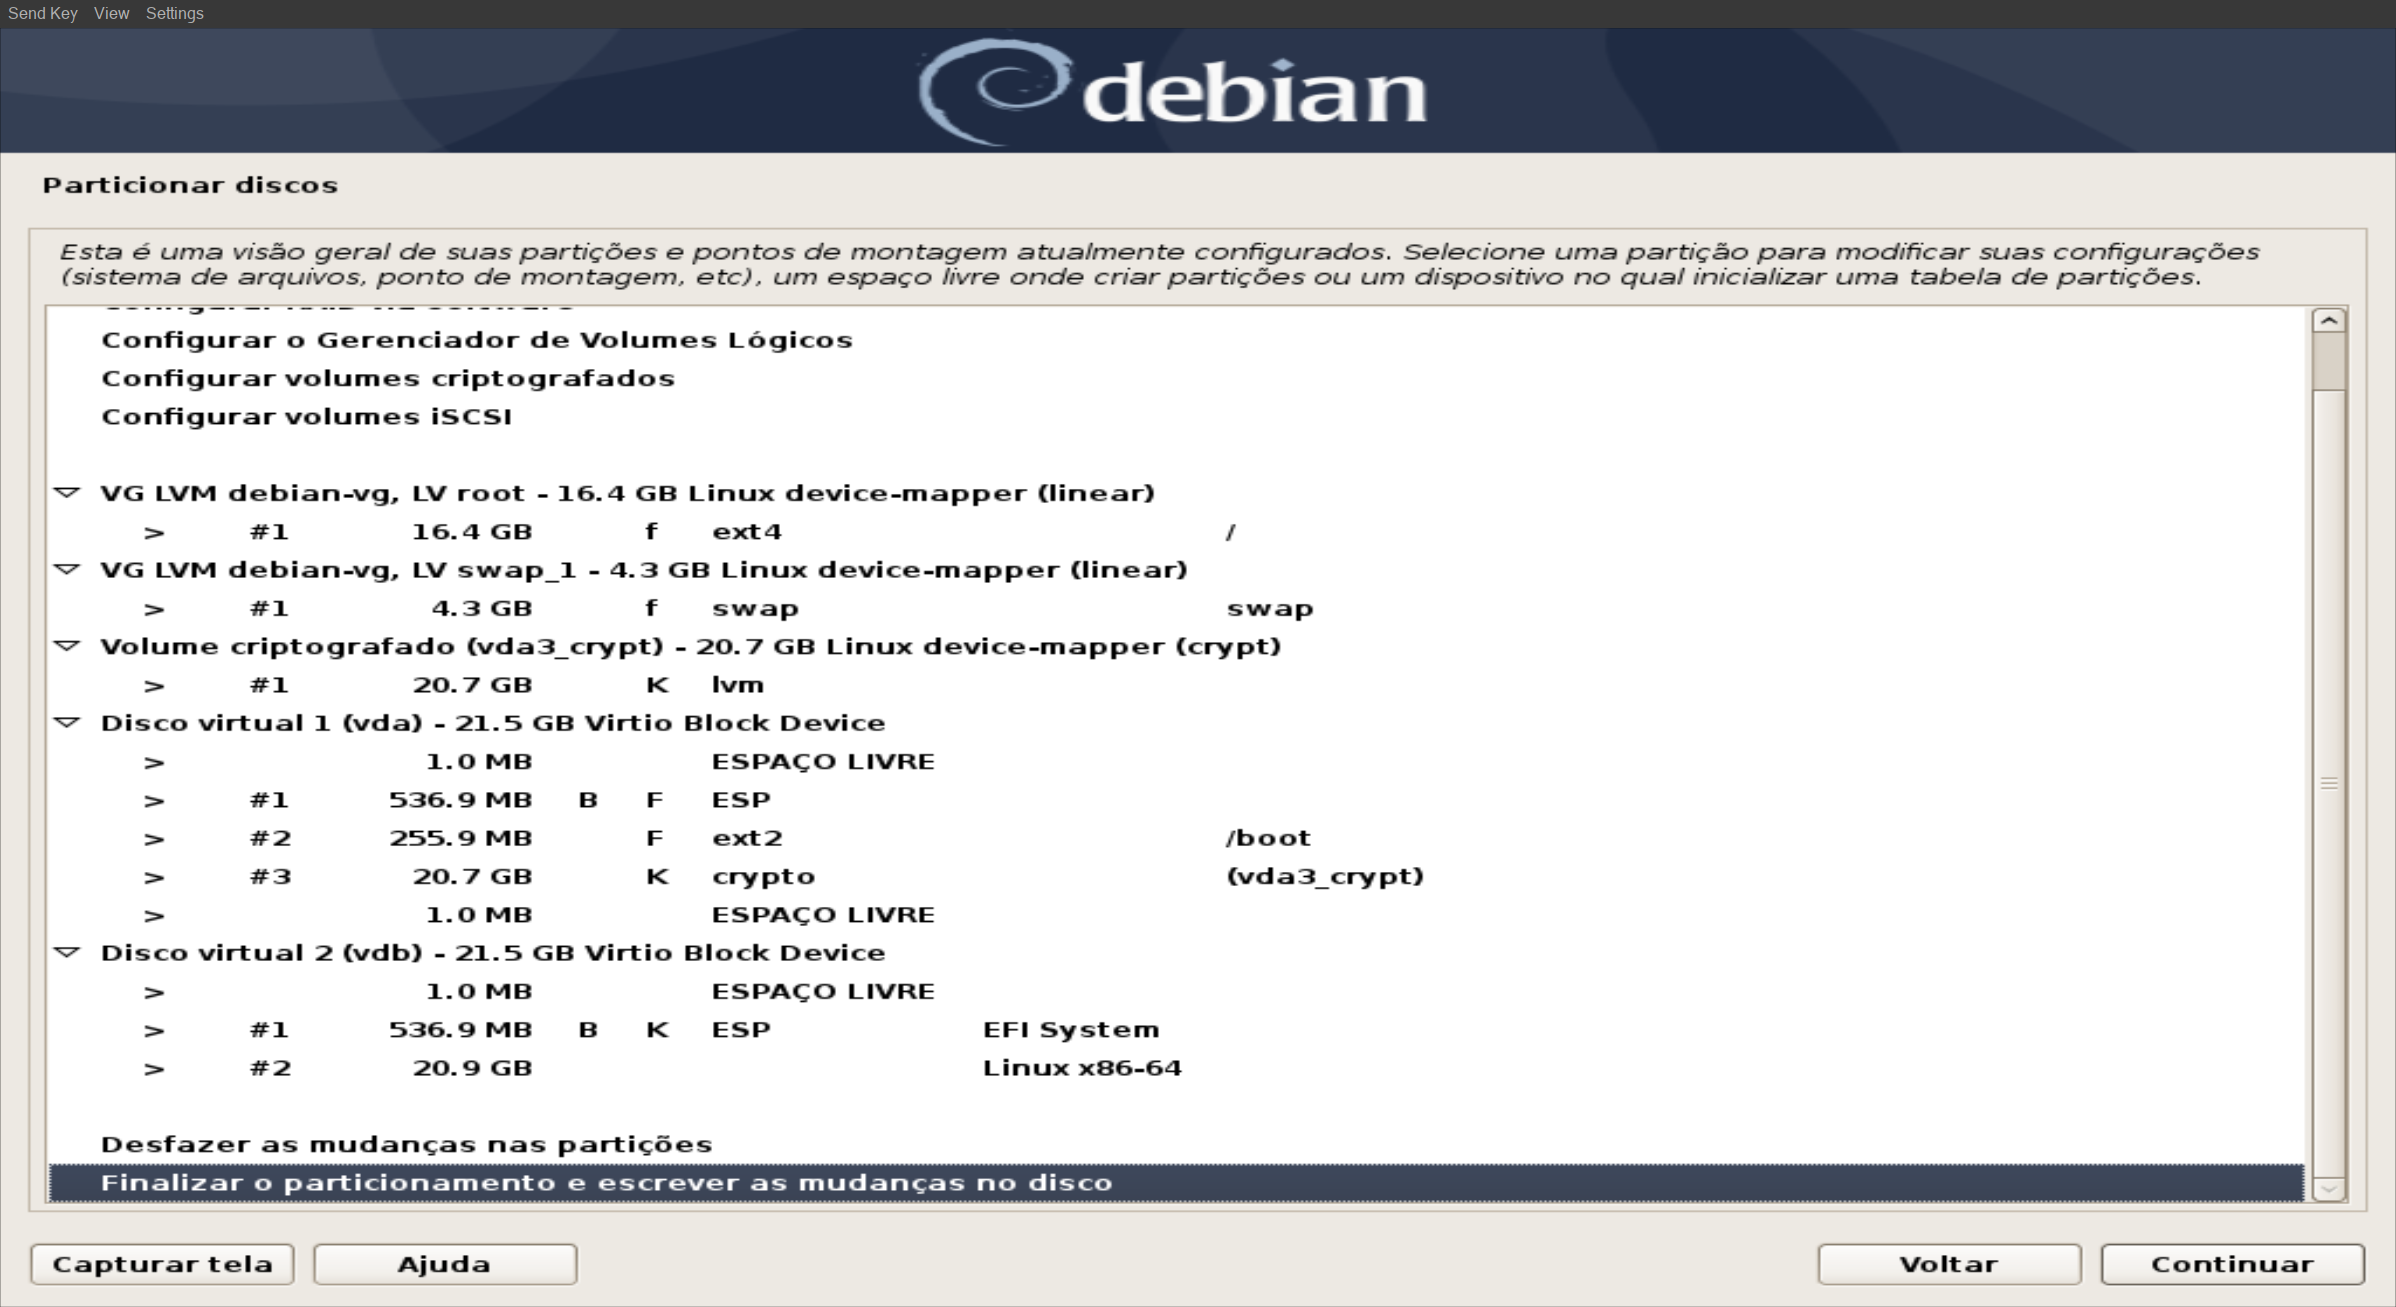
\includegraphics[height=1\textheight, width=.8\linewidth,
  keepaspectratio]{end-encrypt}
  \caption{Finalizar particionamento.}
  \label{fig:end_encrypt}
\end{figure}

O sistema irá formatar os volumes e iniciar a instalação do sistema
operacional para o disco/SSD. Este procedimento levará algum tempo,
então apanha uma xícara de café/chá. Caso você possua um SSD,
provavelmente não terá tempo hábil de apanhá-lo :).

A tela da figura~\ref{fig:end} indica que você instalou com sucesso.
Reinicie conforme passos da tela e siga para a seção~\ref{sec:verify}.


\section{Verificando instalação} \label{sec:verify}
Após feita toda instalação do sistema e iniciado com suas credencias
de criptografia de disco e seu usuário, ou seja, dentro da sua área de
desktop, execute o seguinte comando a partir de um terminal como
usuário \textbf{root}.

\begin{verbatim}
$ dmidecode -t 1,2; blkid

# dmidecode 3.2
Getting SMBIOS data from sysfs.
SMBIOS 3.2.1 present.
# SMBIOS implementations newer than version 3.2.0 are not
# fully supported by this version of dmidecode.

Handle 0x0001, DMI type 1, 27 bytes
System Information
	Manufacturer: Dell Inc.
	Product Name: Inspiron 3583
	Version: Not Specified
	Serial Number: G0CCD33
	UUID: 4c4c4544-0030-4310-8043-c7c04f443333
	Wake-up Type: Power Switch
	SKU Number: 08CA
	Family: Inspiron

Handle 0x0002, DMI type 2, 15 bytes
Base Board Information
	Manufacturer: Dell Inc.
	Product Name: 0DXF6K
	Version: A01
	Serial Number: /G0CCD33/BRFCB0002Q007T/
	Asset Tag: Not Specified
	Features:
		Board is a hosting board
		Board is replaceable
	Location In Chassis: Not Specified
	Chassis Handle: 0x0003
	Type: Motherboard
	Contained Object Handles: 0

/dev/vda1: UUID="4183-67DD" TYPE="vfat" \
PARTUUID="015c7b79-f055-4f25-b1f8-ce089506e144"
/dev/vda2: UUID="d44a3c27-14d7-4efd-a7ab-c7b7dbf6c4f3" TYPE="ext2" \
PARTUUID="f6c1d239-0d67-4747-a316-9980f2609870"
/dev/vda3: UUID="88267bab-0a32-471a-8518-9e19275f5d40" TYPE="crypto_LUKS" \
PARTUUID="fc31265f-dc5f-4492-ba14-908e9dd05ebc"
/dev/mapper/vda3_crypt: UUID="yspPEu-EwNn-enkK-pwDq-Jy2E-qeID-r9eu2h" \
 TYPE="LVM2_member"
/dev/mapper/debian--vg-root: UUID="295cf7dc-f844-4939-84d9-54afe5a9cc37" \
TYPE="ext4"
/dev/mapper/debian--vg-swap_1: UUID="8a4b3194-ab5a-432f-8160-b4006f4162aa" \
TYPE="swap"
\end{verbatim}
 
\textcolor{red}{\textbf{Obs: as informações apresentadas acima poderão variar com o seu sistema.}}\\

Copie e cole a saída dos comandos e envie ao seu gestor.

Parabéns, você instalou e configurou seu sistema Debian!
    \clearpage
  
\end{document}